\documentclass[a4paper]{article}
\usepackage[utf8]{inputenc}
\usepackage{graphicx}

\title{\Large{\textbf{A Brief Survey of Genetic Algorithms}}}
\author{By Robert Bergers}
\date{May 2019}

\begin{document}

\maketitle

% begin abstract
\begin{center}
    \Large{\textbf{Abstract}}
\end{center}
Artificial intelligence is a type of algorithm which allows a computer to take input from an environment which is used to intelligently generate output to achieve a certain goal. While most types of AI algorithms are strictly based off of research in the field of computer science, evolutionary computation is a family of AI algorithms which is heavily inspired by evolutionary biology. Genetic algorithms are a type of evolutionary computation that are based off the principles of evolution at the genetic level. Genetic algorithms faced a lot of academic skepticism in their first few decades, but exponential increase in both computational power and research have made them extremely efficient at solving certain types of problems. This survey paper describes the history of genetic algorithms, how they are implemented and when it is appropriate to do so.
% end abstract

\section{Evolutionary Computation}
% Broad overview of the history of evolutionary computation
\textit{Evolutionary computation} is a set of algorithm paradigms which derive their mechanisms from evolutionary biology. There are three main categories of evolutionary computational algorithms: \textit{genetic algorithms}, \textit{evolutionary programming}, and \textit{evolution strategies}. Genetic algorithms specifically mimic the behaviors biologists have observed in genetic reproduction and evolution.\\

"Although the origins of evolutionary computation can be
traced back to the late 1950’s ... the field remained relatively unknown to the broader scientific community for almost three decades. This was largely due to the lack of available powerful computer platforms at that time, but also due to some methodological shortcomings."\cite{echistory} Even with the modern computational power of computers and highly efficient algorithms, genetic algorithms can take days, weeks or even months to achieve their goals. This means that any modern problem that was solved with genetic algorithms, such as optimizing the fuel efficiency of jet engines, were attempted in the 1950s it would probably still be searching for a solution to this day.\\

Thanks to the Hollands research in genetic algorithms and more available computational power, genetic algorithms began gaining popularity in the 1970s. It was around this time when it was discovered what types of problems genetic algorithms are best at solving. Now they are used by biologists and chemists as well as computer scientists.

\section{Genetic Algorithms}
% Explain how genetic algorithms work, what kinds of problems
% they can be applied to.
Genetic algorithms are most widely known for their efficiency in optimization problems, where the efficiency of each generated solution is easily placed on a slider scale. However, genetic algorithms are also commonly implemented for automatic programming, economic models, immune system models, ecological models, population genetics models and to study the relationship between evolution and learning.\cite{overview}\\

\subsection{Stating the Problem}
% Explain how a problem is defined in such a way that it can
% be solvable with a genetic algorithm
The first step in the process of writing a genetic algorithm to find a solution to a problem is to define the problem in a way that is compatible with the genetic algorithm paradigm.\\

In order for a genetic algorithm to work, there must be a way to identify a \textit{goal state}. This way the genetic algorithm knows what a solution looks like. A \textit{heuristic}, also known as an \textit{objective function} or \textit{fitness function}, is a function applied to each generated solution that determines how close the solution is to the goal state. The GA seeks to generate a solution that optimizes the heuristic for either the minimum or the maximum. Depending on the problem the GA seeks to solve, there may need to be multiple objective functions.\\

Each solution the genetic algorithm generates takes the form of a \textit{chromosome}, a string of bits. Each subsection of the chromosome string that represents a feature of the solution is called a \textit{gene} or \textit{allele}.\\

To give these concepts context, we will apply them to the 8 queens toy problem. The goal of the 8 queens problem is to place 8 queens on a chess board such that no queen can capture another queen.
\begin{itemize}
    \item\textbf{Chromosome}: 1826374452617085
        \begin{itemize}
            This is an example of a solution which is generated and tested by the genetic algorithm
        \end{itemize}
    \item\textbf{Alleles}: 18, 26, 37, 44, 52, 61, 70, 85
        \begin{itemize}
            The chromosome is split into alleles, the individual parts of the solution. In this example, each allele represents the coordinates of a queen.
        \end{itemize}
    \item\textbf{Fitness function}: $x = c_q_1 + c_q_2 + c_q_3 + ... + c_q_8$
        \begin{itemize}
            This is the function which determines how close a chromosome is to the goal state and identifies when the goal state is achieved. $c_{q}$ represents the number of queens each queen is capable of capturing.
        \end{itemize}
    \item\textbf{Goal state}: $x = 0$
        \begin{itemize}
            The goal is to optimize $x$, the total number of queens that can be captured, for the global minimum.
        \end{itemize}
\end{itemize}

\subsection{Selection Process}
% Explain the methods used to select solutions from population
While there are many different approaches to each step in a genetic algorithm, the first is always the same: Generate a random \textit{population} of solutions. Each of the solutions is executed on the problem which runs it through the fitness function. Once the efficiency of each solution is known, the genetic algorithm begins the selection process.\\

The natural equivalent of the selection process is a cornerstone of Darwinian philosophy; 'survival of the fittest'. The less efficient a specimen is in nature, the less likely it is to spread its genes to the next generation.\\

Here are the most common selection methods:
\begin{itemize}
    \item \textbf{Roulette Wheel Selection}
    \begin{itemize}
        Roulette wheel selection is the most randomized method of selection, where any solution in the population has a chance to be selected. The more highly optimized each solution is, the higher its chance of being selected for crossover. If 10 chromosomes in the population have the same fitness, they will all have equal odds of being selected. \cite{gastudyapp}
    \end{itemize}
    \item \textbf{Rank Selection}
    \begin{itemize}
        Rank selection is similar to roulette wheel selection in the sense that any chromosome in a population has a chance of being selected, but the difference is that no two chromosomes have equal chance of being selected. The solutions are ordered by their fitness in an array, and given a rank which increments for each chromosome. The least fit chromosome has a rank of 1, and the most fit has a rank of $N$, the total number of solutions in the population. The higher the rank, the higher the chance of the chromosome being selected for crossover. \cite{gastudyapp}
    \end{itemize}
    \item \textbf{Elitism Selection}
    \begin{itemize}
        Elitism selection is guaranteed to select the fittest solution for crossover, and then implements rank selection or roulette wheel selection for the rest of the selection process. \cite{gastudyapp}
    \end{itemize}
    \item \textbf{Best Selection}
    \begin{itemize}
        Best selection is the only selection method with no element of randomness. This selection process is guaranteed to send the fittest given percentage of the population to the crossover process.
    \end{itemize}
\end{itemize}

\subsection{Crossing Over}
% Explain different methods of crossing over

\begin{figure}[h!]
    \centering
    \begin{subfigure}{\columnwidth}
        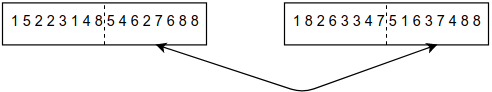
\includegraphics[width=0.8\columnwidth]{singlepoint.png}
        \caption{Single-point crossover}
        \label{singlepoint}
    \end{subfigure}
    \begin{subfigure}{\columnwidth}
        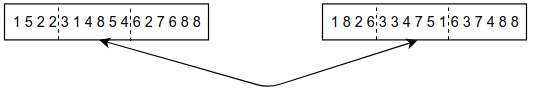
\includegraphics[width=0.8\columnwidth]{doublepoint.png}
        \caption{Two-point crossover}
        \label{twopoint}
    \end{subfigure}
    \begin{subfigure}{\linewidth}
        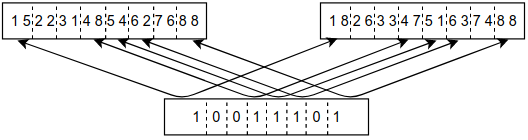
\includegraphics[width=0.8\linewidth]{uniform.png}
        \caption{Uniform crossover}
        \label{uniform}
    \end{subfigure}
\end{figure}

Once the genetic algorithm finishes selecting the fittest solutions, it then begins the process of \textit{crossing over}. This is a concept taken directly from biology. Crossing over occurs in nature during meiotic cell division, where homologous chromosomes link and swap alleles from corresponding genetic loci.\\

There are three main methods of crossing over in genetic algorithms. \textit{Single-point crossover}, illustrated in figure \ref{singlepoint}, splits the selected chromosomes at a random point between two alleles, then swaps the fragments. \textit{Two-point crossover}, illustrated in figure \ref{twopoint}, splits the selected chromosomes at two random points between alleles, then swaps the center fragments. \textit{Uniform crossover}, illustrated in figure \ref{uniform}, splits each chromosome between every allele. It then generates a random binary string with a length equal to the number of alleles in the chromosomes. Every allele in the chromosomes is swapped whose corresponding value in the binary string is 1.

\subsection{Mutations}
% Explain advantages of adding mutation probability
"The mutation operator is used to change some elements in selected individuals with a probability $p_m$ (the mutation rate or mutation probability), leading to additional genetic diversity to help the search process escape from local optimal traps."\cite{adaptcm}\\

The mutation process can take place before, during or after the crossing over process. It adds the chance for an allele to spontaneously change its value. It is worth noting that adding a mutation probability does not necessarily improve the efficiency of a genetic algorithm. A mutation probability typically only improves GA performance if the objective function has many local maximums or minimums.\\

The effectiveness of a mutation rate is also dependent on how many times the crossing over process is executed on a population of chromosomes before the GA gives up and spawns a new random population. If the crossing over process occurs only a few times, then a mutation probability would likely not have any significant impact on the performance of the GA.

\section{GA Benefits and Drawbacks}
% Explain real (and perceived) problems with genetic algorithms
At a certain level of abstraction, genetic algorithms can sound exactly the same as natural genetic evolution. However, in practical application, the connection can be very loose. Observed behaviors of genetic evolution are only implemented in genetic algorithms where it makes sense to do so. For example, a genetic algorithm might only include randomness in the generation of the initial solution population. The selection and crossing over processes might be given strict rules with no element of randomness, and/ or the genetic algorithm might not even have a mutation probability. When genetic algorithms were initially introduced, the idea was that the more similar genetic algorithms were to nature, the more efficient they would be. The amount of truth to this statement varies depending on the problem the genetic algorithm is being used to solve, but it is often far from the truth.\\

There is one important feature that genetic algorithms and natural genetic evolution always have in common: knowing how to solve a problem is not necessary. They both solve problems by recombining the best available solutions into even better solutions. One of genetic algorithms biggest advantages is that unlike most machine learning algorithms, the programmer does not need to have a solid understanding of how to solve a problem before they can write an algorithm to solve the problem.

% Bibliography
\begin{center}
\textbf{References}
\end{center}
\begin{bib}

\bibliography{bib}
\bibliographystyle{plain}

\bibitem[0]{gastudyapp}[0] H. Lingaraj {\em A Study on Genetic Algorithm and its Applications} 2016: International Journal of Computer Sciences and Engineering.

\bibitem[1]{handbook}[1] L. D. Davis {\em Handbook of Genetic Algorithms} 1998.

\bibitem[2]{gaml}[2] D. E. Goldberg, J. H. Holland {\em Genetic Algorithms and Machine Learning} 1988: Kluwer Academic Publishers.

\bibitem[3]{ga}[3] J. H. Holland {\em Genetic Algorithms} 1992: Scientific American.

\bibitem[4]{echistory}[4] T. Back, U. Hammel, H. Schwefel {\em Evolutionary Computation: Comments on the History and Current State} 1997.

\bibitem[5]{adaptcm}[5] W. Lin, W. Lee, T. Hong {\em Adapting Crossover and Mutation Rates in Genetic Algorithms} 2003: Journal of Information Science and Engineering.

\bibitem[6]{overview}[6] M. Mitchell {\em Genetic Algorithms: An Overview} 1995: John Wiley & Sons, Inc.

\end{bib}
\bibliography{sreadings}
\bibliographystyle{plain}
\begin{sreadings}



\end{sreadings}

\end{document}
